\documentclass{beamer}

\usepackage[german]{babel}

\usepackage{tikz}
\usetikzlibrary{trees}

\usetikzlibrary{calc}
\usetikzlibrary{bending}
\usetikzlibrary{decorations.pathreplacing}

\pgfdeclarelayer{bg}
\pgfsetlayers{bg,main}

\tikzset{
	db/.pic={
		\draw[white, fill=white](-.6,0) rectangle (.6,1.4);
		\draw[white, fill=white](0,1.4) ellipse [x radius=.6,y radius=.15];
		\foreach \y in {0,.5,1}
		{
			\draw[thick, fill=white]
				(-0.6,\y) to [looseness=0.5,bend right=90] ++(1.2,0)
						  to ++(0,0.4)
						  to [looseness=0.5,bend left=90] ++(-1.2,0)
						  to ++(0,-0.4);
			\draw[thick] (-0.6,\y+0.4) edge[looseness=0.5,bend left=90] ++(1.2,0);
		}
	}
}


\title{Git \& \textrm{\LaTeX}-Einführung}
\author{
    Noah Kälin\inst{1},
    Simon Walker\inst{1},
	Naoki Pross\inst{1}
}
\institute[HSR]{\inst{1}Hochschule f\"ur Technick Rapperswil}

\date{24. September / 1. Oktober 2019}

\usetheme{Malmoe}
\usecolortheme{seagull}

\AtBeginSection[]
{
	\begin{frame}[shrink]{Inhaltsverzeichnis}
		\tableofcontents[
			currentsection,
			hideothersubsections,
			sectionstyle=show/shaded,
		]
	\end{frame}
}

\begin{document}

\frame{\titlepage}

\section{Warum Git}

\begin{frame}{Was brauchen wir?}
	\begin{block}{Das Problem}
		Dateien zwischen Machine synchronisieren und sie mit mehr Leute
		bearbeiten. Spezifischer Textdateien bearbeiten (z.B. Quellcode)
	\end{block}
	\pause

	\begin{block}{Eine L\"osung}
	\centering
	\vspace{1em}
	
\includegraphics[width=0.25\textwidth]{pic/git.png}\\
	\vspace{1em}

	(Engl. f\"ur Bl\"odmann) Entwickelt von Linus Torvalds
	\end{block}
\end{frame}

\begin{frame}{Was ist git?}
	\begin{block}{Was wir brauchen}
	\begin{itemize}
		\item Synchronisation
		\item Team Datei Bearbeitung
		\item Problemlose Offline-Nutzung
	\end{itemize}
	\end{block}
	\pause

	\begin{block}{Was kriegen wir extra}
	\begin{itemize}
		\item Geschichte jedes Dokuments im Projekt
		\item Kryptographische Sicherheit der Projektgeschichte
		\item Gemeinsamer Dateizugriff ohne zentraler Server 
	\end{itemize}
	\end{block}
\end{frame}

\begin{frame}[c]{Bemerkung}
	\centering
	{\LARGE 
	Git l\"ost ein komplex Problem \\
	daher ist Git auch komplex
	}

	{\footnotesize
		But don't worry it's not \emph{too} hard
	}
\end{frame}
\end{frame}

\begin{frame}{Arbeitsablauf}
	Arbeitsablauf um eine Formelsammlung zu bearbeiten (alleine).
	\begin{enumerate}
		\item Fork ein Repository von HSR-Stud \pause
		\item Bearbeiten \pause
		\item Fortlaufend Commits erstellen Bsp. nach jedem Kapitel \pause
		\item Push
	\end{enumerate}
	
\end{frame}

\begin{frame}{Arbeitsablauf II}
Arbeitsablauf um eine Formelsammlung zu bearbeiten (mehrere Autoren).
\begin{enumerate}
	\item Fork ein Repository von HSR-Stud  \pause
	\item Jede Person erstellt einen Branch \pause
	\item Bearbeiten \pause
	\item Fortlaufend Commits erstellen Bsp. nach jedem Kapitel \pause
	\item Mit dem Master mergen Bsp. nach jedem Kapitel \pause
	\item Push
\end{enumerate}

\end{frame}

\section{\LaTeX}

{\setbeamertemplate{background canvas}{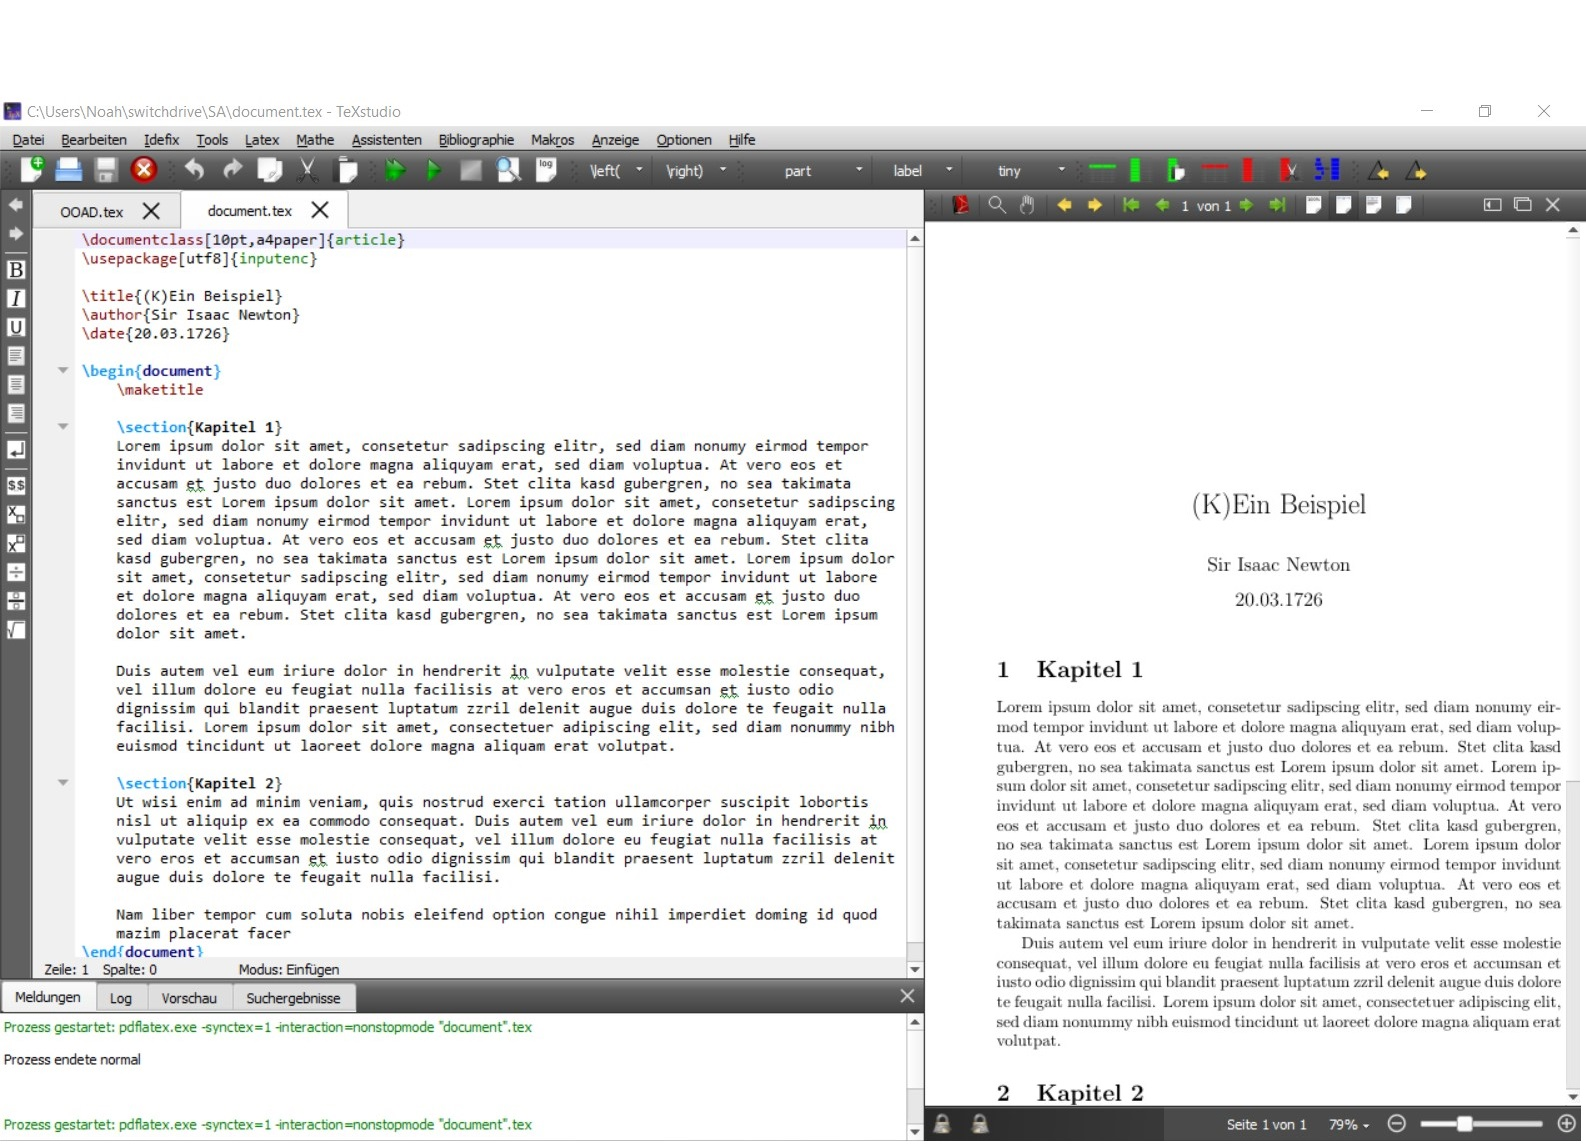
\includegraphics[width=\paperwidth]{pic/bild}}
\begin{frame}

\end{frame}
}

\begin{frame}
	\begin{itemize}
		\item \LaTeX: \textbf{La}mport \textbf{TeX} 
		\item TeX: Textsatzsystem 
		\item Kein WYSIWYG sondern WYSIWYAF
	\end{itemize}
\end{frame}

\begin{frame}{Warum \LaTeX?}
\begin{itemize}
	\item Open-Source 
	\item Grosse Community 
	\item Performance 
	\item Kein WYSIWYG 
	\item Professionell 
	\item Wissenschaftliche Formeln 
	\item Cross-Platform
\end{itemize}
\end{frame}


\end{document}
